\documentclass[12pt]{article}
\usepackage{amsmath, amssymb}
\usepackage{geometry}
\geometry{a4paper, margin=1in}
\usepackage{setspace}
\usepackage{lmodern}
\usepackage{graphicx}
\usepackage{titlesec}

% Formatting section headings
\titleformat{\section}[block]{\bfseries\Large}{\thesection.}{1em}{}
\titleformat{\subsection}[block]{\bfseries\large}{\thesubsection.}{1em}{}

\title{Question 2: Statistical Analysis of Antithyroid Hormone Levels}
\author{}
\date{}

\begin{document}
\maketitle
\onehalfspacing

\section*{Problem Statement}
Alice suffers from a thyroid disorder. The concentration of antithyroid hormone in her blood is described by the following observations.

\bigskip

\section*{Part 1: Mean and Quartiles}
Let the number of observations be:
\[
n = 14.
\]
The data in ascending order is:
\[
x_1 = 0.11, \quad x_2 = 1.44, \quad \dots, \quad x_i, \quad \dots, \quad x_n = 10.8, \quad i \in \{1,2,\dots,n\}.
\]

The mean is calculated as:
\[
\bar{x} = \frac{1}{n} \sum_{i=1}^{n} x_i = \frac{2613}{700} \approx 3.733.
\]

The indices for the quartiles are:
\[
\begin{alignedat}{2}
i_{Q_1} &= \frac{n}{4}+\frac{1}{2} &= 4, \\
i_{Q_2} &= \frac{n}{2}+\frac{1}{2} &= 7.5, \\
i_{Q_3} &= \frac{3}{4}n+\frac{1}{2} &= 11.
\end{alignedat}
\]

The first quartile ($Q_1$), median ($Q_2$), and third quartile ($Q_3$) are determined as:
\[
\begin{alignedat}{3}
Q_1 &= \frac{x_{\lceil i_{Q_1}-\frac{1}{2} \rceil} + x_{\lfloor i_{Q_1}+\frac{1}{2} \rfloor}}{2} &= x_4 &= 2.6, \\
Q_2 &= \frac{x_{\lceil i_{Q_2}-\frac{1}{2} \rceil} + x_{\lfloor i_{Q_2}+\frac{1}{2} \rfloor}}{2} &= \frac{x_7 + x_8}{2} &= 3.615, \\
Q_3 &= \frac{x_{\lceil i_{Q_3}-\frac{1}{2} \rceil} + x_{\lfloor i_{Q_3}+\frac{1}{2} \rfloor}}{2} &= x_{11} &= 4.38.
\end{alignedat}
\]

\textbf{Answer for Part 1:}
\[
\bar{x} = \frac{2613}{700} \approx 3.733, \quad Q_1 = 2.6, \quad Q_2 = 3.615, \quad Q_3 = 4.38.
\]

\bigskip

\section*{Part 2: Boxplot}
The minimum and maximum values are:
\[
\begin{aligned}
\text{min} &= x_1 = 0.11, \\
\text{max} &= x_n = 10.8.
\end{aligned}
\]

The corresponding boxplot is displayed below:

\begin{center}
    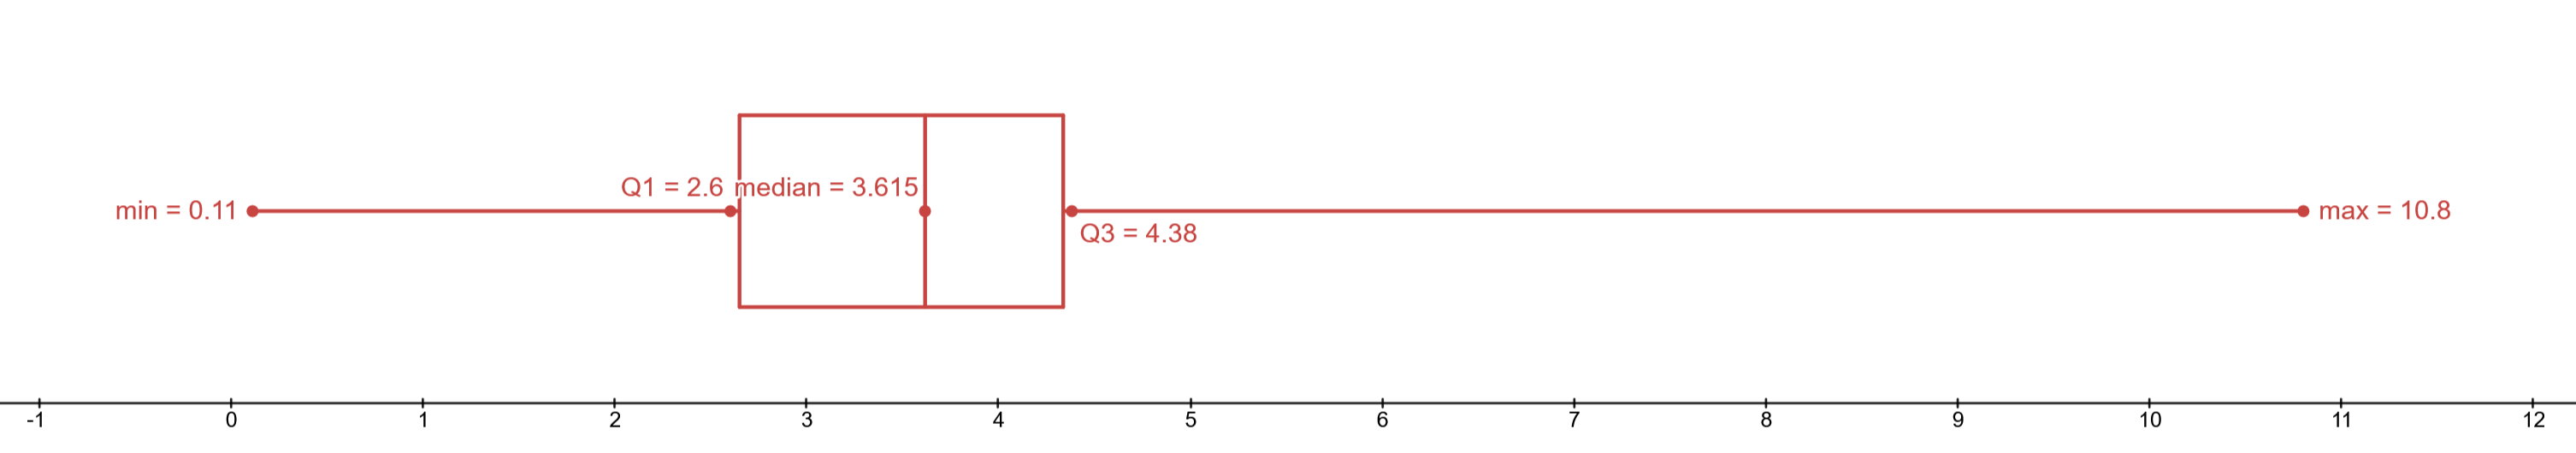
\includegraphics[width=1\textwidth]{Q2-P2-boxplot.png}
\end{center}

\textbf{Answer for Part 2:} Boxplot is shown above.

\end{document}
